\documentclass[12pt]{article}
\usepackage{amsmath,amsfonts,fullpage,amsthm,graphicx,verbatim}

\newtheorem*{theorem}{Theorem}
\newtheorem*{fact}{Fact}
\newtheorem*{goal}{Goal}
\newtheorem*{idea}{Idea}
\newtheorem*{defn}{Definition}
\newtheorem*{ex}{Example}

%Style section
%\setlength{\textheight}{10in}
%\setlength{\textwidth}{7in}
%\hoffset=-0.75in
 \pagestyle{plain}
% \setlength{\topmargin}{0in}
% \setlength{\headsep}{0in}
% \setlength{\oddsidemargin}{0in}
% \setlength{\evensidemargin}{0in}

\begin{document}


\pagestyle{empty} %use this to get rid of page numbers

\noindent
{Math 166  \hskip 1.5 truein  Names:\ \hrulefill}

\noindent
%\vskip 0.3truein
%\bigskip
%\noindent
{Trig substitution}

\noindent  \hskip 3.5 truein  Section Number:\ \hrulefill
\smallskip

\begin{goal} \rm
Trig substitution: making integrals simpler (or at least doable) 
\end{goal}
\begin{enumerate}
\begin{comment}
	
\setcounter{enumi}
\item (Trig review) Write down expressions for $\tan$, $\cot$, $\sec$, and $\csc$ in terms of $\sin$ and $\cos$.
\vspace{1.25in}
\item Starting with everyone's favorite trig identity, $\sin^2 x + \cos^2 x = 1$, do some algebraic manipulation to write down two different identities involving $\tan^2$, $\cot^2$, $\sec^2$, and/or $\csc^2$. (Hint: we found one of these identities in class yesterday)
\vspace{1.25in}


\item Evaluate the integral by the following steps.
\[\displaystyle\int  \frac{1}{x^4\sqrt{x^2-4}} \ dx\]
\begin{enumerate}
\item First, substitute $x=2\sec(\theta)$ (this is a \emph{trig substitution}). Convert the integral completely into the variable $\theta$. (Hint: If $x=2\sec(\theta)$ then what does $dx$ equal?) 

\vspace{1.25in}
\item Use the trig identity $\tan^2(\theta)+1=\sec^2(\theta)$ to simplify the denominator by making the part under the square root into a perfect square. (This kind of simplification is the goal of trig substitution.) Then evaluate the integral.


vfill
\vfill
\vfill

\item Convert back to the variable $x$ by using our trig substitution $\sec(\theta)=\frac{x}{2}$ and the definition of the trig functions in terms of a right triangle.

\medskip
\begin{center}
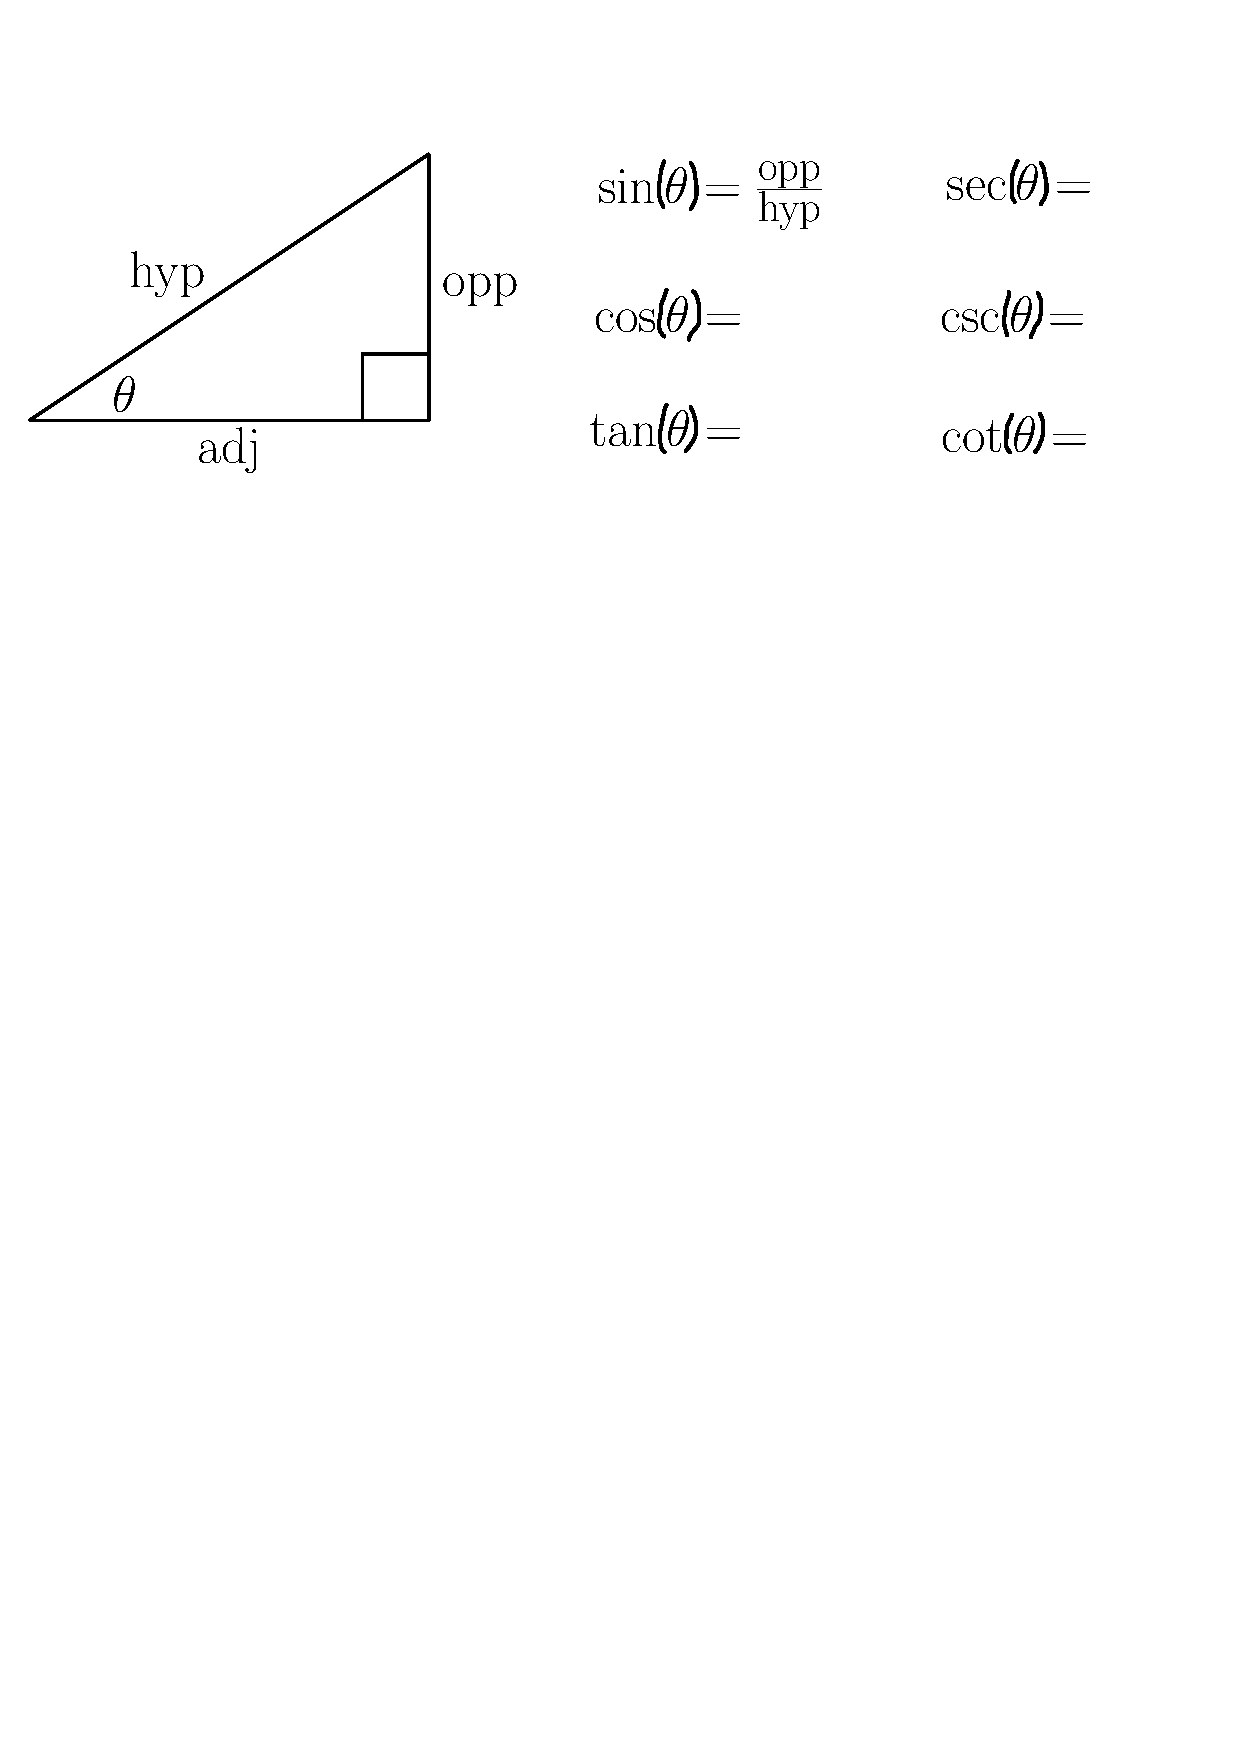
\includegraphics[scale=.65]{right_triangle.pdf} 
\end{center}

\item Write your answer in terms of the variable $x$.

\end{enumerate}
\end{comment}

%\item What trig substitution should you use if your integrand contains $\sqrt{x^2-a^2}$? Why?
%\bigskip

%\item What trig substitution should you use if your integrand contains $\sqrt{x^2+a^2}$? Why?
%\bigskip

%\item What trig substitution should you use if your integrand contains $\sqrt{a^2-x^2}$? Why?

%\vspace{1.5cm}
%\newpage
\item Evaluate the integral by the following steps.
\[\displaystyle\int  \frac{x}{(x^2-6x+5)^{5/2}} \ dx\]
\item Complete the square in the denominator.
\[x^2-6x+5 =(x^2-6x+\underline{~~~} \ )+5-\underline{~~~}=(x-3)^2-\underline{~?~}
\]

\vspace{1cm}
\item Now make the substitution $u=x-3$ to get the integrand into a form where we can use trig substitution. Convert the integral completely into the variable $u$.

\vspace{1.25in}

\item Now set $u$ equal to something involving a trig function of $\theta$ that will turn the expression in the denominator into a perfect square.
%set $u=2\sec\theta$ (this is the trig substitution). 
Convert the integral completely into the variable $\theta$. (Hint: What does $du$ equal in terms of $\theta$?) 

\vspace{1.25in}
\item Use the trig identity $\sin^2(\theta) + \cos^2(\theta) = 1$ or $\tan^2(\theta)+1=\sec^2(\theta)$ to simplify the denominator. (This kind of simplification is the goal of trig substitution.)

\vspace{2in}

\item The resulting trig integral is: \[\displaystyle\int  \frac{(2\sec(\theta)+3)(2\sec(\theta)\tan(\theta))}{32\tan^5(\theta)} \ d\theta.\] (If what you have so far is not equivalent to this, go back and check your work and/or ask your TAfor help.) Multiply out the numerator and simplify to obtain the two integrals: \[\displaystyle\frac{1}{8}\displaystyle\int  \frac{\sec^2(\theta)}{\tan^4(\theta)} \ d\theta + \frac{3}{16}\displaystyle\int\frac{\sec(\theta)}{\tan^4(\theta)} \ d\theta.\]

\vfill
\item Evaluate these trig integrals. You will need to use more substitutions (use a new variable, like $w$) and trig identities. If you don't see what substitution to use, you may try converting the secants and tangents to sines and cosines. The answer in terms of $\theta$ is $\frac{-1}{24}\cot^3(\theta)-\frac{1}{16}\csc^3(\theta)+\frac{3}{16}\csc(\theta)+C$.

\vfill
\newpage

\item Convert back to the variable $u$ by using our chosen trig substitution %$\sec\theta=\frac{u}{2}$ 
and the definition of the trig functions in terms of a right triangle.
\begin{center}
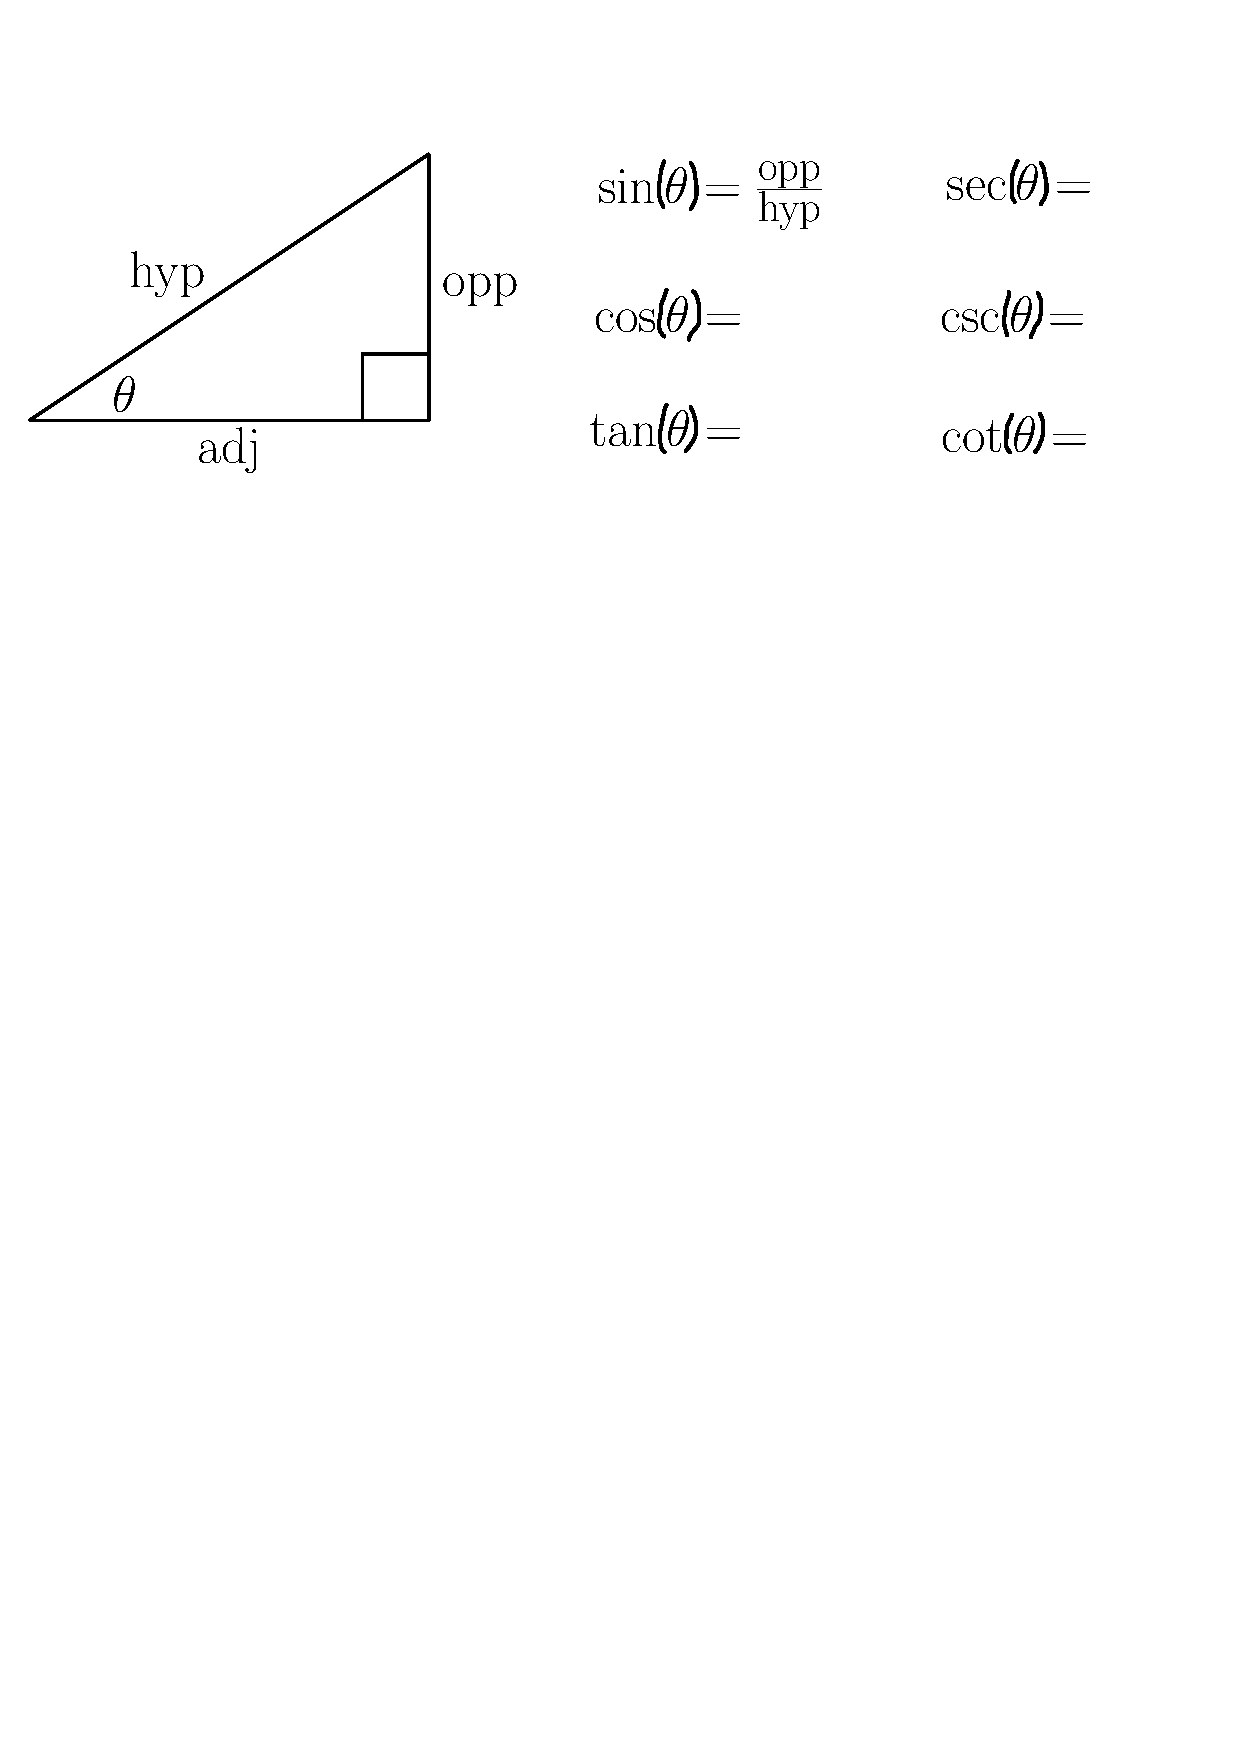
\includegraphics[scale=.45]{right_triangle.pdf} 
\end{center}
\vfill

\item Write your answer in terms of the variable $x$.

\vfill

\end{enumerate} 

\end{document}
